\documentclass{article}
\setlength{\oddsidemargin}{0.25 in}
\setlength{\evensidemargin}{-0.25 in}
\setlength{\topmargin}{-0.6 in}
\setlength{\textwidth}{6.5 in}
\setlength{\textheight}{8.5 in}
\setlength{\headsep}{0.75 in}
\setlength{\parindent}{0 in}
\setlength{\parskip}{0.1 in}

\newtheorem{theorem}{Theorem}
\newtheorem{corollary}{Corollary}
\newtheorem{proposition}{Proposition}
\newtheorem*{remark}{Remark}
\theoremstyle{definition}
\newtheorem{example}{Example}
\newtheorem{definition}{Definition}

\newcommand{\lecture}[4]{
   \pagestyle{myheadings}
   \thispagestyle{plain}
   \newpage
%   \setcounter{lecnum}{#1}
   \setcounter{page}{1}
   \noindent
   \begin{center}
   \framebox{
      \vbox{\vspace{2mm}
    \hbox to 6.58in { {\bf CSC~565: Graph Theory
                        \hfill North Carolina State University} }
    \hbox to 6.58in { {\bf Fall 2019
                        \hfill Computer Science} }
       \vspace{4mm}
       \hbox to 6.28in { {\Large \hfill Lecture #1: #2  \hfill} }
       \vspace{2mm}
       \hbox to 6.28in { {\it Lecturer: {\it Don Sheehy {\tt <drsheehy@ncsu.edu>}} \hfill Scribe: #4} }
      \vspace{2mm}}
   }
   \end{center}
   \markboth{Lecture #1: #2}{Lecture #1: #2}
   \vspace*{4mm}
}

\usepackage{amsmath,latexsym,amsbsy,amssymb}
\usepackage{graphicx}
\newtheorem{definition}{Definition}
\newtheorem{lemma}{Lemma}
\begin{document}
    \lecture{16}{Oct 16, 2019}{Don Sheehy}{Carl Klier, Nuhal Ravindra, Shahil Shah, Erica Swain }
    \begin{lemma} If a graph $G$ is 3-connected and $|V_{G}|>4$ then, there exists an edge $e\in E_{G}$ such that $G / e$ (graph G where edge e is contracted) is 3-connected.
    \end{lemma}
    
    Suppose there is a graph that is 3-connected and has 4 vertices. It will always be $k_{4}$. 
    \\
    \centerline{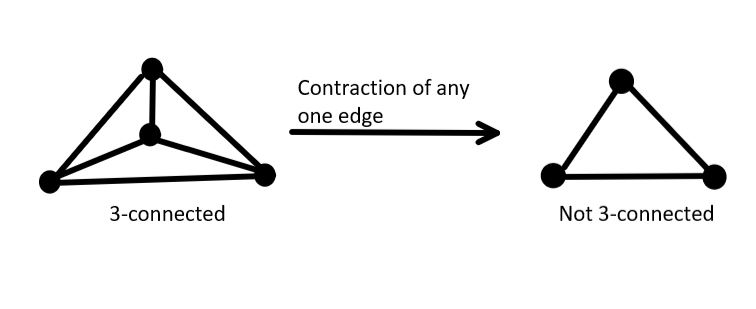
\includegraphics[width=5in]{Images/k4.jpg}}
    \\
    \subsubsection*{\underline{\textbf{Proof of Lemma 1}} :}
    We try to prove lemma 1 using contradiction.
    \\\\
    Suppose that for any edge $(x,y)$ that we choose, if we contract the edge then the graph is no longer 3-connected. There will also be an another vertex $z$ such that if we also add $z$ to the cut set, the graph will be separated. Suppose the graph is separated into two not necessarily connected pieces.
    \\\\
    Now we choose $e = (x,y)$ and $z$ such that we minimize $|A|$ i.e. the size of number of vertices in A.
    \\\\
    Also there must be a vertex $v$ in A such that there is an edge $(v,z)$ otherwise $z$ won't be in the cut set.
    \\\\
    Similarly there must be a vertex w having an edge incident to it as $(z,w)$ so that we can get a cut set $ \{z,v,w\} $ which separates the graph.
    \\\\
    Every vertex in B has a path that goes to $x$ and a disjoint path that goes to $y$ otherwise the graph would have been just 2-connected and not 3-connected. Here $w$ could have been either $x$ or $y$.  
    \\\\
    Let us assume that $w \neq x$ without any loss of generality.
    \\\\
    So $\exists$  path from $b$ to $x$ in $G \backslash \{ z,v,w \}$ where $b$ can be any vertex in the piece B.
    \\\\
    We can see that the component of $G \backslash \{ z,v,w \}$ that does not contain $x$ or $y$ is a subset of A.
    \\\\
    We chose $x,y,z$ to minimize $|A|$ but we got an even smaller component and so a contradiction!
    \\\\
    \centerline{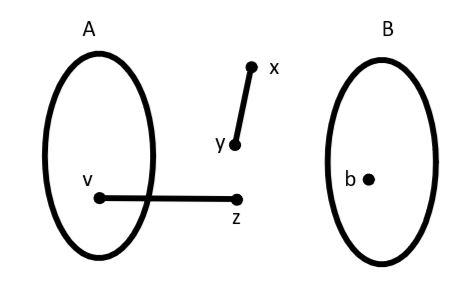
\includegraphics[width=3in]{Images/lemma1.jpg}} 
    \\\\
    
    \subsubsection*{Fary's Theorem Proof Recap : }
    \centerline{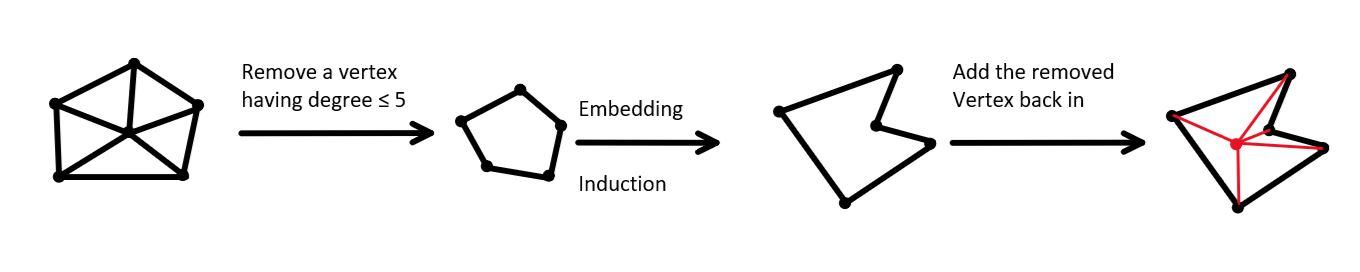
\includegraphics[width=7in]{Images/Fary.jpg}} 
    \newpage
    \section*{Kuratowski/Wagner theorem for 3-connected graphs : }\begin{lemma}
        If a graph $G$ is 3-connected and does not contain $k_{5}$ and $k_{3,3}$ minors, then $G$ is planar 
    \end{lemma}
    \subsubsection*{\underline{\textbf{Proof of Lemma 2}} :}
    $\exists e = (x,y)$ such that $G \backslash e$ is also 3-connected.
    \\\\
    By induction $\exists$ an embedding of $G \backslash e$.
    \\\\
    Now if we remove the contracted edge, the result is 2-connected where every face is a cycle.
    \\\\
    Let $C$ be the cycle bounding face. Let $V_{C}$ be the set of all vertices forming the cycle $C$. Let $N(x)$ be the set of all neighbouring vertices of $x$ in $V_{C}$ and $N(y)$ be the set of all neighbouring vertices of $y$ in $V_{C}$. So, $N(x) \cap V(y) \subseteq V_{C}$.
    \\\\
    \underline{\textbf{Claim}} : $ |N(x) \cap N(y)|<3$
    \\\\
    \underline{\textbf{Proof}} : 
    Consider some face with two vertices $x$ and $y$ inside and at least 3 vertices on the face, then if we have  $ |N(x) \cap N(y)| \geq 3$, we get a graph having $k_{5}$ topological minor as shown in the figure below : 
    \\\\
    \centerline{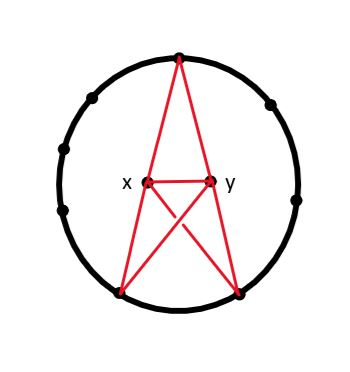
\includegraphics[width=2in]{Images/k5.jpg}} 
    Hence by contradiction we can say that $ |N(x) \cap N(y)|<3 $.
    \\\\
    If we have a cycle in which two vertices $x$ and $y$ are inside it such that the neighbours of $x$ and $y$ on the cycle are in alternating order as shown in following figure then it has a $k_{3,3}$ topological minor. So not having a $k_{3,3}$ as a topological minor means not having an alternating pattern of neighbours.
    \\\\
    \centerline{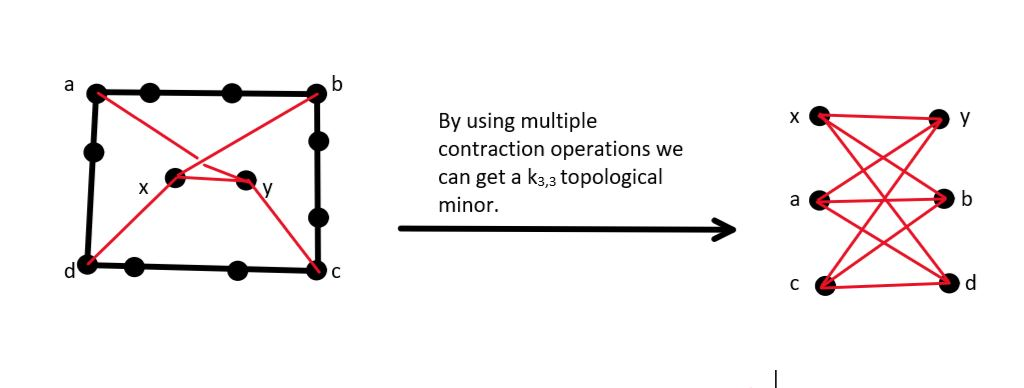
\includegraphics[width=6in]{Images/k3,3.jpg}}
    \\\\
    So finally we can have a cycle where all neighbours of vertex $x$ are followed by all neighbours of vertex $y$ and they might overlap where they meet as shown in following figure. (It is not necessary that all of the vertices on the cycle are neighbours of either vertex $x$ or vertex $y$)
    \\\\
    \centerline{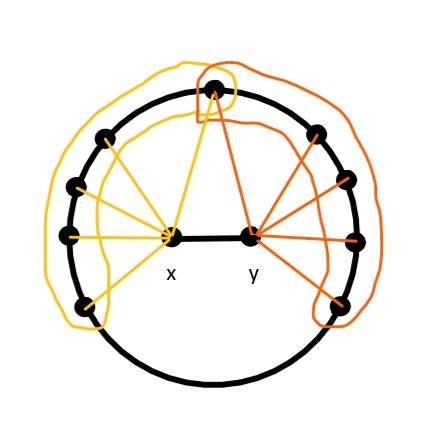
\includegraphics[width=3in]{Images/final_lemma_2.JPG}}
    So we can say that if the graph is 3-connected and does not have $k_{5}$ and $k_{3,3}$ minors then it is definitely planar !
    \newpage
    \underline{\textbf{Claim}} : If a graph has no $k_{5}$ and $k_{3,3}$ minors and is not connected, then it is planar. 
    \\\\
    \underline{\textbf{Proof}} : 
    If the graph is not connected then it has different components where each one is smaller than the whole graph. By induction each of them has an embedding and in the end we can just put them together in a bigger embedding. Suppose we have have two components as follows :
    \\\\
    \centerline{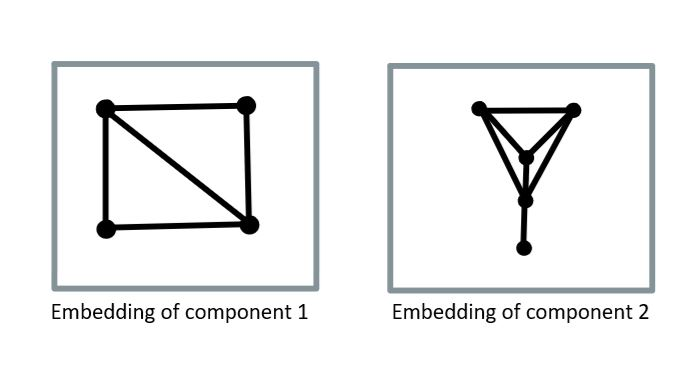
\includegraphics[width=5in]{Images/component_embeddings.JPG}}
    \\\\
    Now we want to put them together into one embedding. One solution is to just take a bigger plane or we can move the components in the plane as shown in other figure.
    \\\\
    \centerline{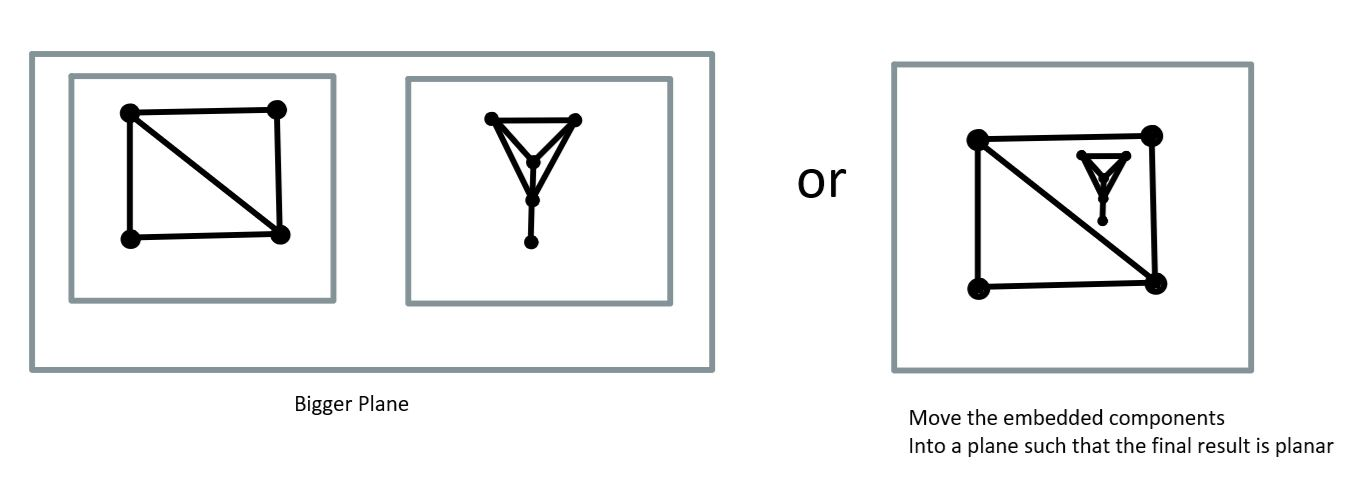
\includegraphics[width=7in]{Images/0_connected_embedding.JPG}}
    \newpage
    \underline{\textbf{Claim}} : If a graph has no $k_{5}$ and $k_{3,3}$ minors and is 1-connected, then it is planar. 
    \\\\
    \underline{\textbf{Proof}} : If the graph is 1-connected then it  can be divided into 2 sub-graphs (A and B) with one vertex as common as shown in the figure. By induction each of the sub-graph has an embedding and in the end we can just glue them together at the common vertex in a bigger embedding.  
    \\\\
    \centerline{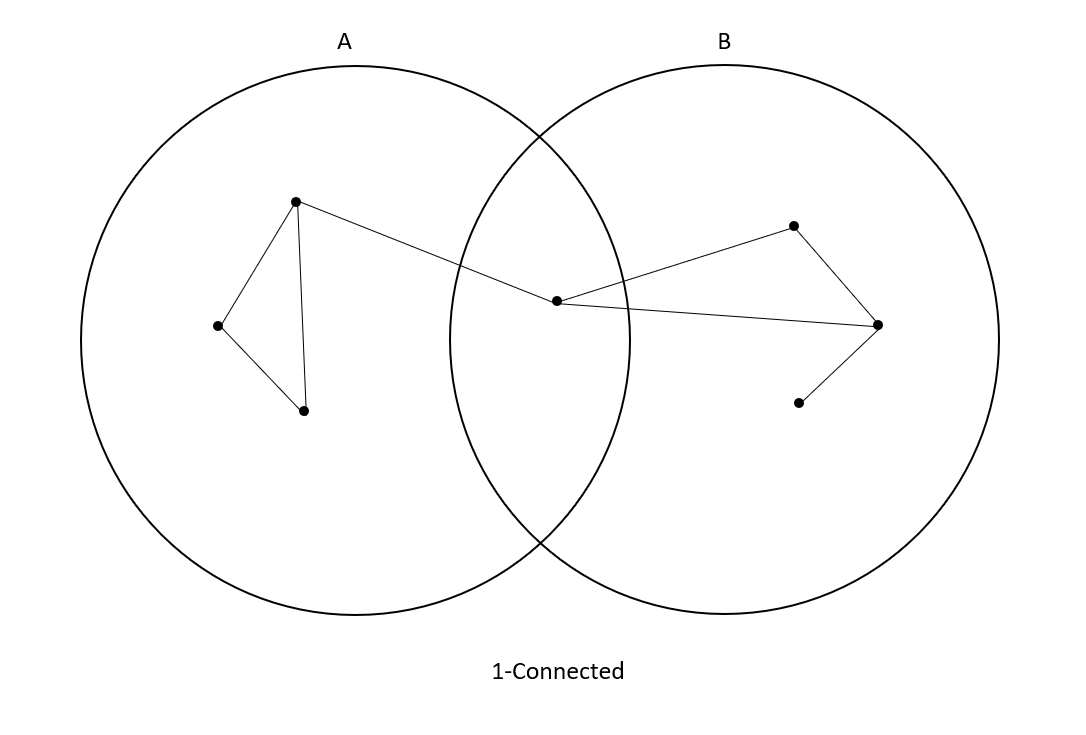
\includegraphics[width=4in]{Images/1conngrapg.PNG}}
    \\\\
    \underline{\textbf{Claim}} : If a graph has no $k_{5}$ and $k_{3,3}$ minors and is 2-connected, then it is planar. 
    \\\\
    \underline{\textbf{Proof}} : If the graph is 2-connected then it  can be divided into 2 sub-graphs (A and B) with one edge in common as shown in the figure. Now we can contract $B \backslash \{x,y\}$ to $x$. The resulting graph has fewer vertices than original and if the original did not contain edge $(x,y)$, the new graph will have one. We can do the same thing where we contract $A \backslash \{x,y\}$ to x. Now we can embed these two newly formed graphs and glue them together at edge $(x,y)$. Also it is always possible to glue them together at edge $(x,y)$ because for both graphs we can select an outer face which contains the edge $(x,y)$.
    \\\\
    \centerline{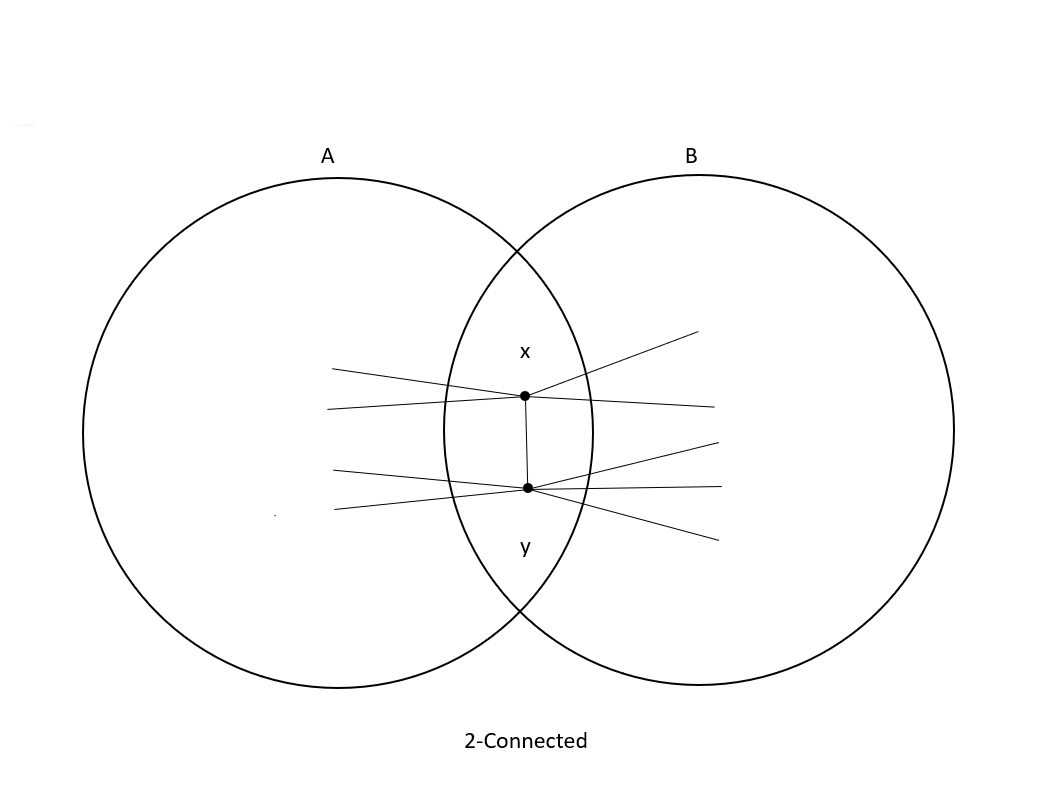
\includegraphics[width=4in]{Images/2conngraph.PNG}}
    \newpage
    \section*{Duals of a planar graph : }
    First let's talk about the map coloring problem. The problem states that is it possible to color every region of a map such that no to neighbouring region are colored with the same color?
    \\\\
    The map coloring theorem states that we can always do it by using at most 4 colors.Though it might not be possible if we have a disconnected region or when the dual of the map is not planar. 
    \\\\
    We can create a dual of a map by having one vertex per region of the map and having edges between adjacent regions. This is shown in following figure  :
    \\\\
    \centerline{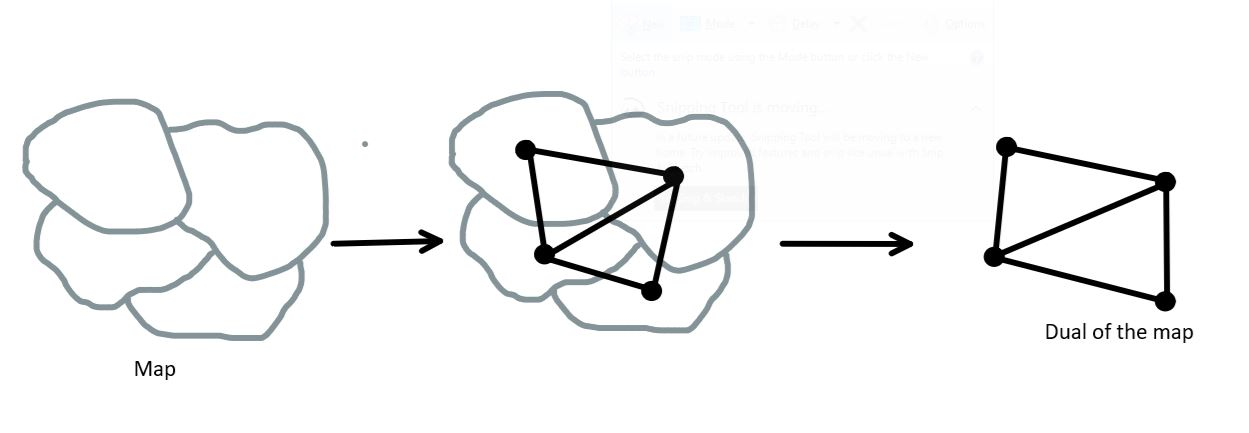
\includegraphics[width=6in]{Images/map_coloring.JPG}}
    (Here we have not considered a vertex for the outermost unbounded region but for duals of graphs which we will see later, that has to be considered !)
    \\\\
    If the dual of a map is not planar then we cannot color the whole map using at most 4 different colors.
    \\\\
    Consider following figure : 
    \\\\
    \centerline{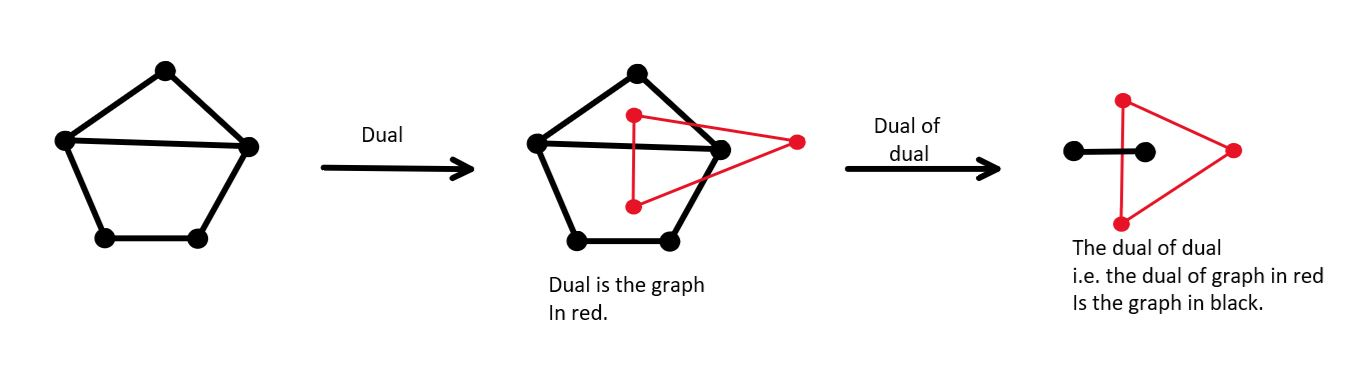
\includegraphics[width=6in]{Images/dual_1.JPG}}
    Here we can see that the dual of dual for a 2-connected graph does not necessarily gives us the original graph from which we started.
    \\\\
    Suppose we allow multiple edges between vertices i.e. let us assume that a multigraph is possible.
    \\\\
    \centerline{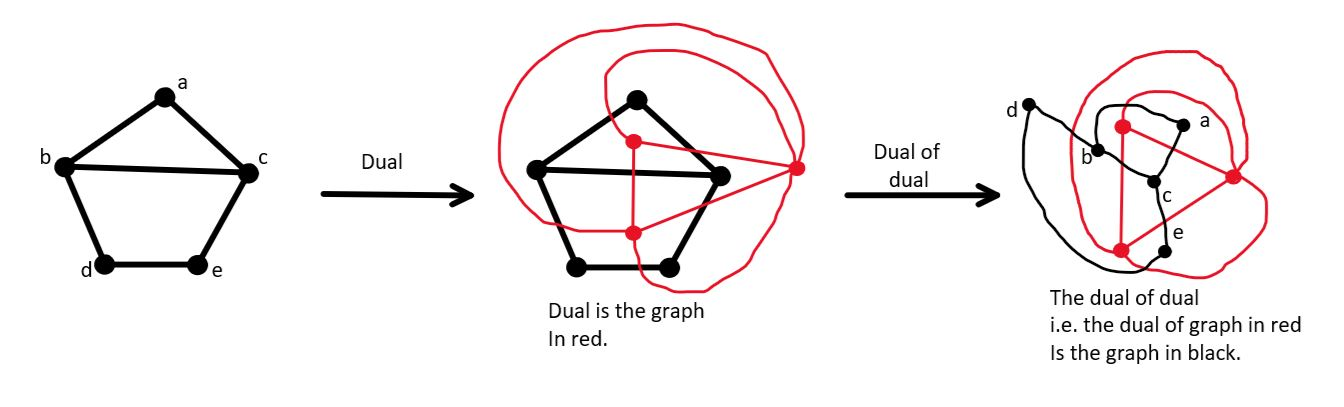
\includegraphics[width=6in]{Images/dual_2.JPG}}
    As we can see in above picture that if we allow multiple edges, we can get the same graph back by dualing twice.
    \\\\
    Now let's talk about duals for 3-connected planar graphs. A primal is the graph that we originally started with and a dual is the graph that we end up after performing the dual operation. For a 3-connected planar graph the faces in primal are one to one mapped to vertices in dual, vertices in primal are one to one mapped to faces in dual and as euler's formula holds true the edges in primal are one to one mapped to edges in dual. Also if we apply dual operation again to the obtained dual graph, then we get back the graph that we started with i.e. the primal graph.
    \begin{align*}
        &\text{V = vertices in primal ,  V' = vertices in dual} \\
        &\text{F = faces in primal ,  F' = faces in dual} \\
        &\text{E = edges in primal ,    E' = edges in dual }\\\\
        \end{align*}
        We have a mapping of the form : \\\\
        \begin{equation}V \leftrightarrow F'     \end{equation}\\
        \begin{equation} E \leftrightarrow E' \end{equation} \\
        \begin{equation} F \leftrightarrow V' \end{equation}
    \\\\
    Consider a cubic graph which is a 3-connected planar graph. It has 6 faces where each face is bounded by 4 edges. It has 12 edges in total and 8 vertices. The relation between the faces, edges and vertices is shown in following figure : 
    \\\\
    \centerline{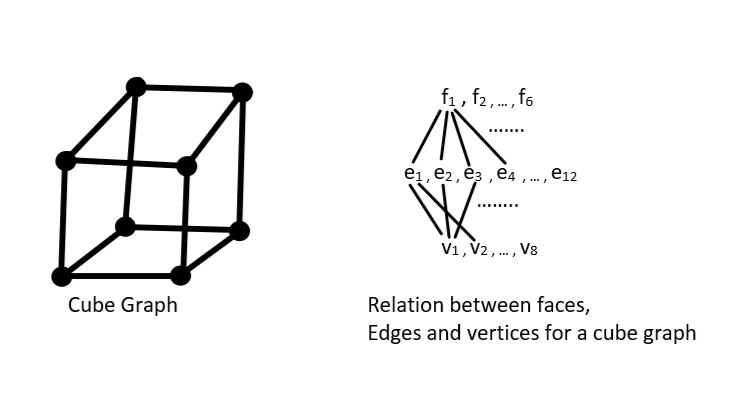
\includegraphics[width=5in]{Images/cube_graph.JPG}}
    \\\\
    Now if we turn this relation in above figure upside down we get a dual which will have a one to one relationship with it's primal i.e. the cube graph for vertices, edges and faces as seen above in equations (1),(2) and (3).
    \\\\
    The dual of cube graph above is : 
    \\\\
    \centerline{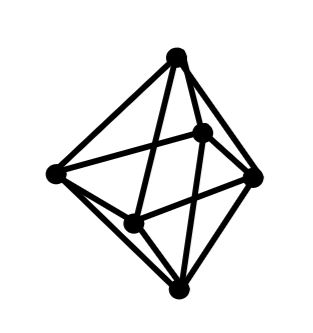
\includegraphics[width=2in]{Images/octahedron.JPG}}
    \newpage
    \textbf{Reciprocal Diagrams - James Clerk Maxwell}
    \\\\
    Forces acting on an object can be rearranged to form a polygon by gluing the forces end-to-end where the forces get canceled out when in a equilibrium. This is known as \textbf{Force Polygon}.
    \\\\
    \centerline{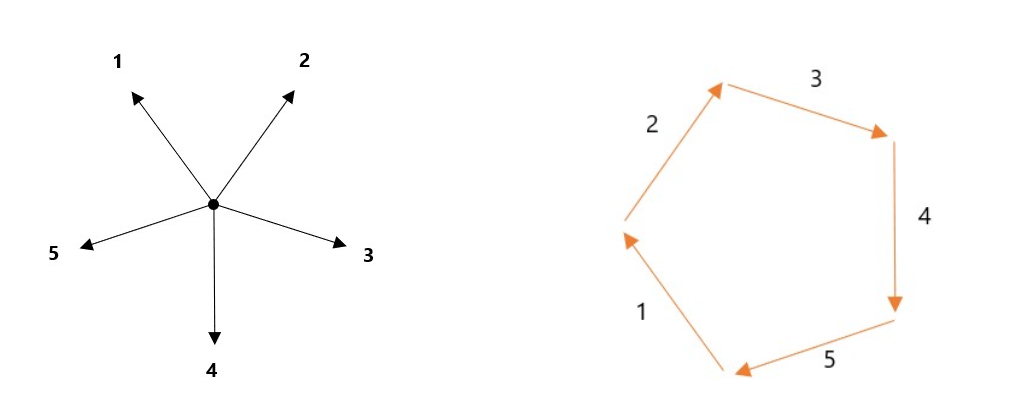
\includegraphics[width=7in]{Images/forcegraph.png}}
    \\\\
    Here the diagram depicts the forces in equilibrium acting on an object and these forces can be rearranges to form a force polygon. 
    \\\\
    Further, when the forces are applied to a point where the forces are not is equilibrium then the force can be arranged in the form of a polygon, but here the forces are directing to a point as the forces are not in equilibrium.
    \\\\
    \centerline{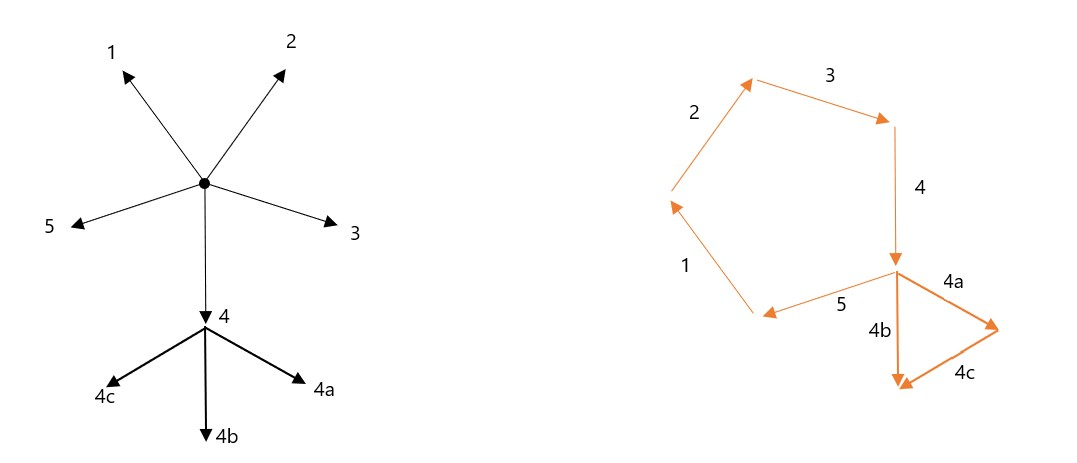
\includegraphics[width=7in]{Images/forcegraphext.jpg}}
    \\\\
    
\end{document}
